% http://tex.stackexchange.com/questions/11866/compile-a-latex-document-into-a-png-image-thats-as-short-as-possible#11880
%http://tex.stackexchange.com/questions/152247/best-practice-to-include-standalone-precompiled-graphics
\documentclass[border=1pt]{standalone}
\usepackage{tikz}

\begin{document}

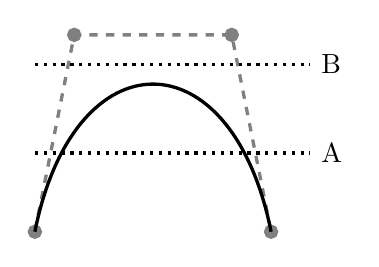
\begin{tikzpicture}[very thick]
	\newcommand {\fy}{2.5}
	\coordinate (p1) at (0,0); \coordinate (p2) at (0.5,\fy);
	\coordinate (p3) at (2.5,\fy); \coordinate (p4) at (3,0);
	\draw[dashed, gray] (p1) -- (p2) -- (p3) -- (p4);
	\foreach \x in {p1,p2,p3,p4}
	{
		\draw[fill=white, gray] (\x) circle [radius=2pt];
	}
	\draw (p1) .. controls (p2) and (p3) .. (p4);
	\draw[dotted] (0,0.4*\fy) -- (3.5,0.4*\fy) node[right] {A};
	\draw[dotted] (0,0.85*\fy) -- (3.5,0.85*\fy) node[right] {B};
\end{tikzpicture}

\end{document}
